\documentclass{article}
\usepackage[utf8]{inputenc}
\usepackage[margin=1in,includefoot]{geometry}
\usepackage{graphicx}
\usepackage{subcaption}
\usepackage{enumerate}
\usepackage{xfrac}
\usepackage{url}
\usepackage{amsmath}
\usepackage{mathtools}
\usepackage{blindtext}
\usepackage[numbers,sort&compress]{natbib}
\usepackage{listings}
\usepackage{color}
\lstset{language=Matlab,
basicstyle=\ttfamily,
keywordstyle=\color{blue}\ttfamily,
stringstyle=\color{red}\ttfamily,
commentstyle=\color{green}\ttfamily,
morecomment=[l][\color{magenta}]{\#}
}
\usepackage{multicol}
\begin{document}
\begin{titlepage}
	\begin{center}
	\line(1,0){450}\\
	[0.25in]
	\huge{\bfseries 3F1 Flight Control Report} \\
	[0.25in]
     \large Investigation on control methods of a simulated aircraft model \\
     \line(1,0){450} \\
	[12cm]
	\textsc{\Large Xiaoding Lu \\[1cm] xl402 \\ Pembroke College \\[1.2cm] 12.10.2018}\\
	\end{center}
	\begin{flushright}

	\begin{figure}[htp]
	\begin{flushright}
	\end{flushright}
	\end{figure}
	\end{flushright}

	\vspace{2cm}

\end{titlepage}

\cleardoublepage
\pagenumbering{roman}
%\tableofcontents
\cleardoublepage
\pagenumbering{arabic}
\section{Overview}
In order to analyse and optimize a real time control system, a mixture of discrete-time and continous-time concepts are used. In this experiment, the plant is an aeroplane with predefined models of dynamics, the plant is discrete-time while the manual controller acts in continous time. Block diagram shown in figure \ref{fig:block} shows the set up of our simple aeroplane control system with nomenclators defined as follows:
\begin{enumerate}
	\item $r(t)$: Reference signal, set to be 0 (horizon) for our experiment
	\item $e(t)$: Error signal
	\item $u(t)$: Controller output
	\item $d(t)$: Input disturbances
	\item $x(t)$: Plant (aeroplane) input
	\item $y(t)$: Plant (aeroplane) output
\end{enumerate}

\begin{figure}[htp]
	\centering
	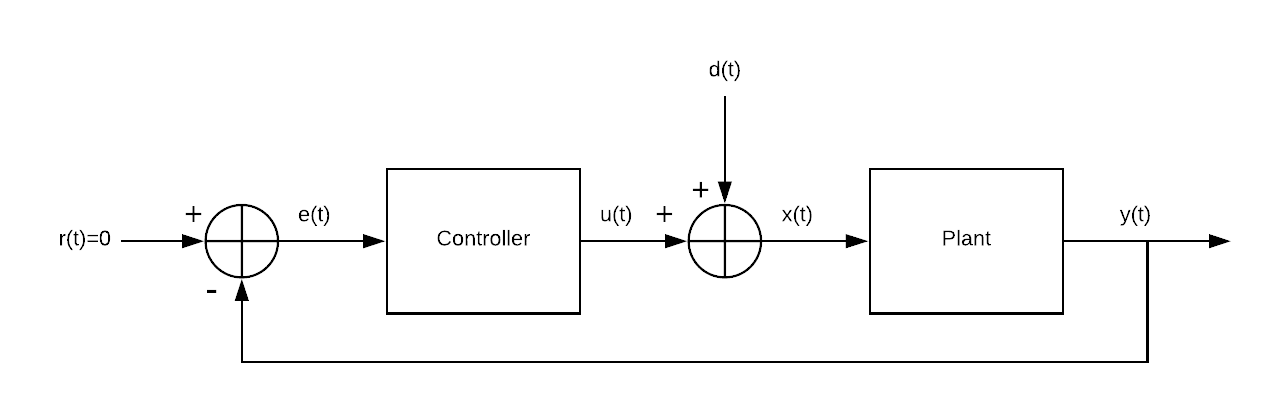
\includegraphics[width=0.9\linewidth]{block_diagram.png}
	\caption{Aeroplane control block diagram}
	\label{fig:block}
\end{figure}
In order to investigate different methods of control (manual, PID) over different models of the aircraft (naturally stable, unstable), we devise a series of investigations below:
\begin{enumerate}
	\item Manual control of the aircraft
	\item Pilot induced oscillation
	\item Sinusoidal disturbances
	\item Unstable aircraft model
	\item Proportional feedback controller
	\item PID controller
\end{enumerate}

\section{Manual Controller Behaviour Analysis}
Starting with a simplified aircraft mode; defined by:
\begin{equation}
	\ddot{y}(t)+M\dot{y}(t)=Nx(t)
\end{equation}
Where $M$ is a coefficient of aerodynamic damping and $N$ is a coefficient of aerodynamic effectiveness of the elevators. The laplace transfer function of this plane is therefore:
\begin{equation}
	G = \dfrac{N}{s^2+Ms}
\end{equation}
Now we need to model and estimate the parameters of the manual controller, figure \ref{fig:manual_control} depicts a typical response graph of a user to a impulse disturbance of magnitude 5 (units) so that $d(t)=5\delta(0)$, note from the previous block diagram in figure \ref{fig:block}, as the reference siganl is always set to zero, the plant output is $y(t)$ is identical to the negative of the error signal $e(t)$, in our case they are interchangable.
\begin{figure}
\centering
\begin{subfigure}{.5\textwidth}
  \centering
  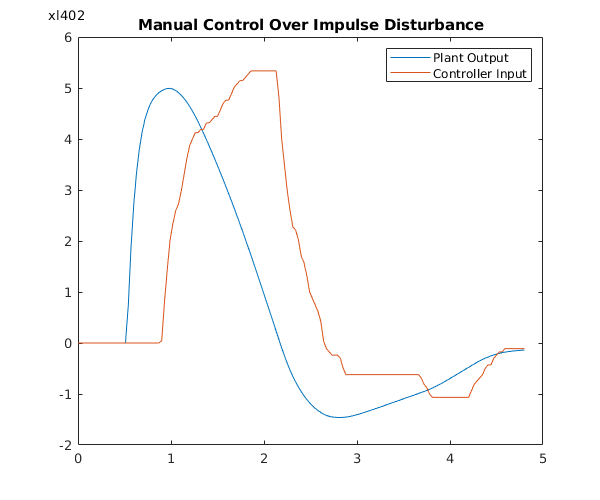
\includegraphics[width=1.1\linewidth]{1_manual_control_input_disturbance.png}
  \caption{Typical response graph}
  \label{fig:manual_control}
\end{subfigure}%
\begin{subfigure}{.5\textwidth}
  \centering
  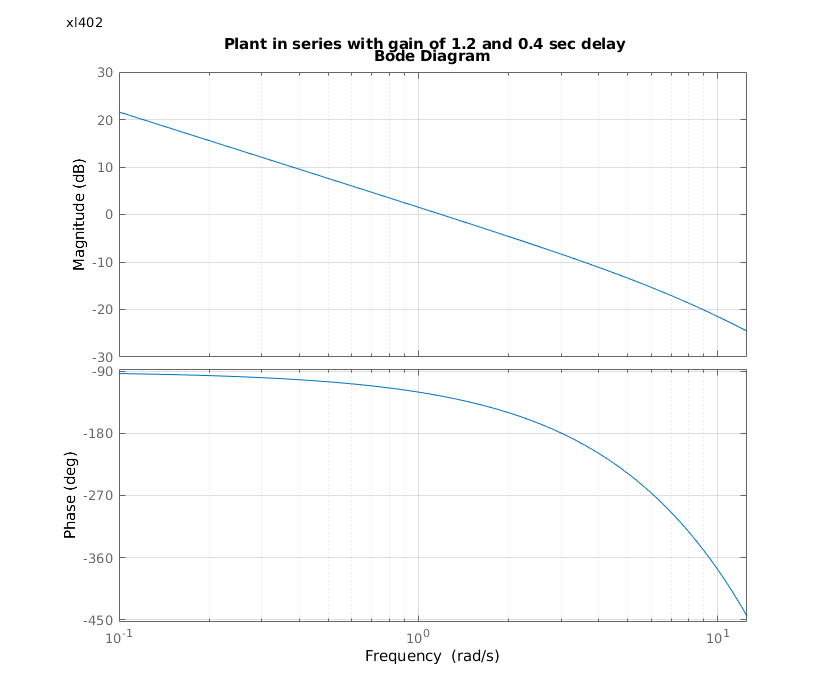
\includegraphics[width=1.1\linewidth]{1_1_Plant_Bode_Manual_Control.png}
  \caption{Open loop Bode plot}
  \label{fig:manual_bode}
\end{subfigure}
\caption{Manual Control}
\label{fig:test}
\end{figure}

A simple model for the manual controller is a proportional gain $k$ in series with a pure time delay $D$. The laplace transfer function of this controller is:
\begin{equation}
	K(s) = ke^{-sD}
\end{equation}
From the response graph in figure \ref{fig:manual_control}, we can estimate parameter $k$ and $D$ where $k$ is estimated as the step impulse the pilot applies after experiencing the impulse disturbance divided by the magnitude of the disturbance, in our case it is:
\begin{equation}
	k = 5.5/5=1.1
\end{equation}
the time delay is read off the x axis to be
\begin{equation}
	D = 0.25 \;\textrm{seconds}
\end{equation}

The Bode diagram for the open loop including the controller is plotted in figure \ref{fig:manual_bode}, from which we can estimate the phase margin by finding the phase corresponding the $0dB$ gain and measure its distance to $180$ degrees. The phase margin estimate is $\phi=50 \textrm{degrees} = 0.87\textrm{rad}$. Hence the amount of extra time delay in this control loop would tolerate before going unstable is:
\begin{equation}
	t_{\textrm{tolerance}} = \dfrac{\phi}{\omega} = 0.87/1.1 = 0.79 \;\textrm{seconds}
\end{equation}
Where $\omega$ is the frequency at which the gain is $0dB$. Figure \ref{fig:nyquist_manual} shows the Nyquist diagram sketched from the Bode plot. Some key points are: we know as $\omega \rightarrow 0$, $\phi \rightarrow 90$ so the plot starts from the bottom right quadrant. The gain margin is approximataly $4dB$ hence the Nyquist x axis intercept in the left quadrant is $-1/4 \approx -0.25$ (the magnitude of this Nyquist plot is also in units of $dB$). Lastly, the magnitude and phase are always decreasing.


\begin{figure}
\centering
\begin{subfigure}{.5\textwidth}
  \centering
  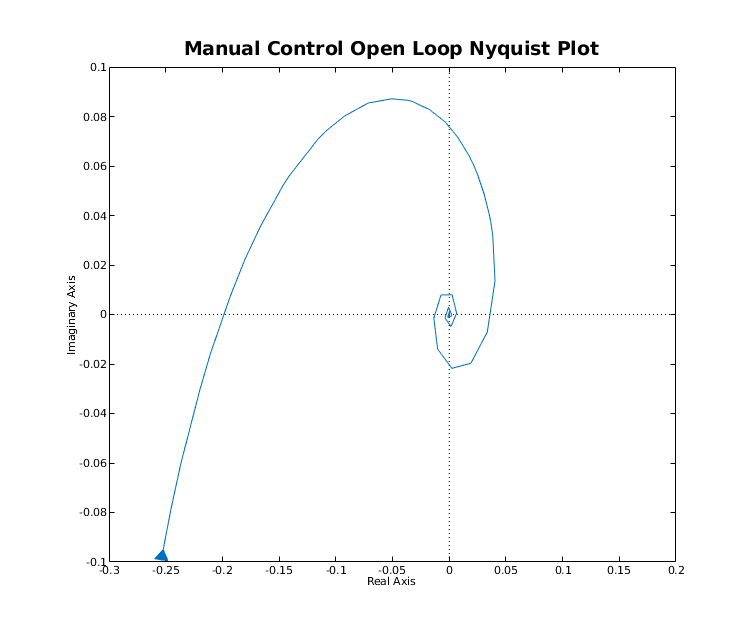
\includegraphics[width=0.8\linewidth]{nyquist_manual.png}
	\caption{Nyquist diagram of open loop control}
	\label{fig:nyquist_manual}
\end{subfigure}%
\begin{subfigure}{.5\textwidth}
  \centering
  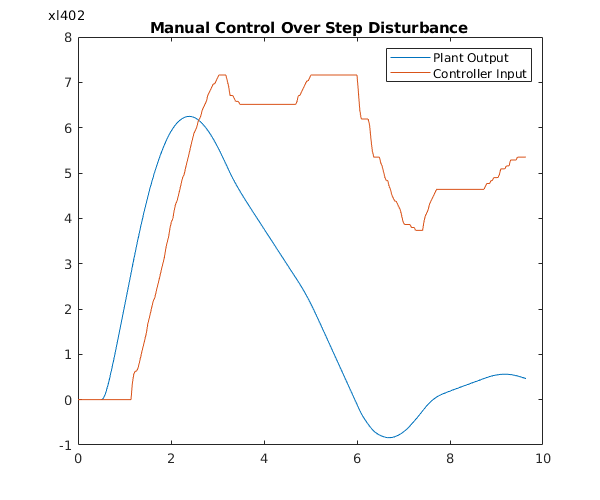
\includegraphics[width=0.8\linewidth]{1_3_Plant_Bode_Manual_Control_Step.png}
  \caption{Typical manual step response}
  \label{fig:step_manual}
\end{subfigure}
	\caption{Manual control responses}
\end{figure}

The basic aircraft model is given a step disturbance of magnitude 5, a typical step response of manual control is depicted in figure \ref{fig:step_manual}, we can see that integral is used, since there is a near constant gradient in the gain, this is to compensate for the fact that the error signal does not decrease as quickly enough (since it is a step instead of an impulse disturbance).

\begin{figure}
\centering
\begin{subfigure}{.5\textwidth}
  \centering
  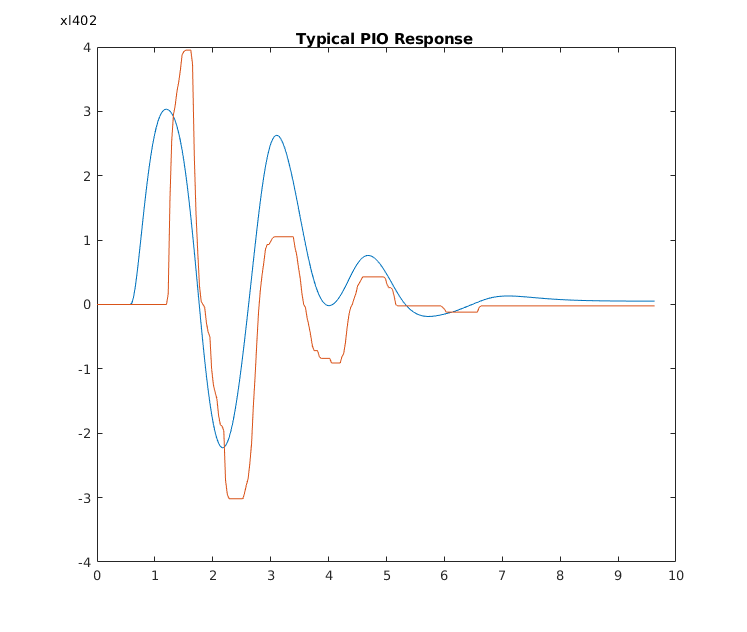
\includegraphics[width=0.8\linewidth]{2_2_PIO_Response_With_Input.png}
	\caption{Typical pilot plant PIO responses}
	\label{fig:pio_response}
\end{subfigure}%
\begin{subfigure}{.5\textwidth}
  \centering
  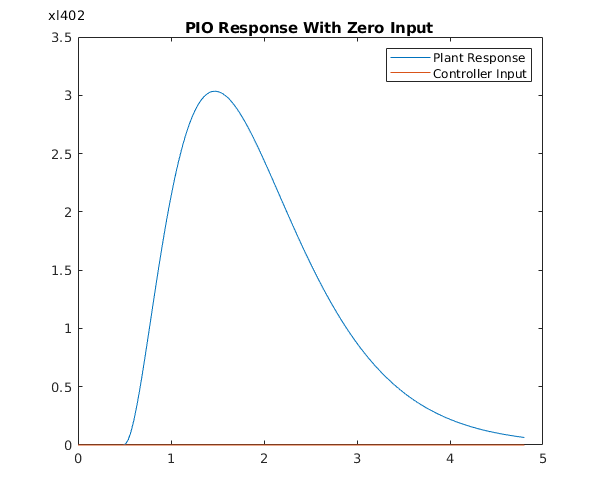
\includegraphics[width=0.8\linewidth]{2_1_PIO_Response.png}
  \caption{Plant response with zero input}
  \label{fig:pio_no_input}
\end{subfigure}
\caption{PIO behaviour analysis}
\end{figure}


\section{Pilot Induced Oscillation Analysis}

A badly designed airraft has the following plant transfer function:
\begin{equation}
	G_1(s)=\dfrac{c}{(Ts+1)^3}
\end{equation}
With parameters $T=4D/pi$ and $c=\sqrt{8}/k$, $k$ and $D$ are gain and time delay of the controller (pilot) modeled previously. A system designed like this, exhibits a phenominom called \textit{pilot induced oscillation}, figure \ref{fig:pio_response} depicts a typical pilot-plant behaviour when the aircraft undergoes a impulse disturbance. Figure \ref{fig:pio_no_input} depicts the plant behaviour under the impulse disturbance without pilot input. We can see that the aircraft is naturally stable, but the pilot's intention to stabalize the aircraft actually causes oscillatary behaviour. To under stand this, the open loop bode plot is shown in figure \ref{fig:pio_bode} is generated with a suitable frequency range, we can see that the phase margin is merely $2$ degrees. This explains why the aircraft is very oscillatary.


\begin{figure}[htp]
	\centering
	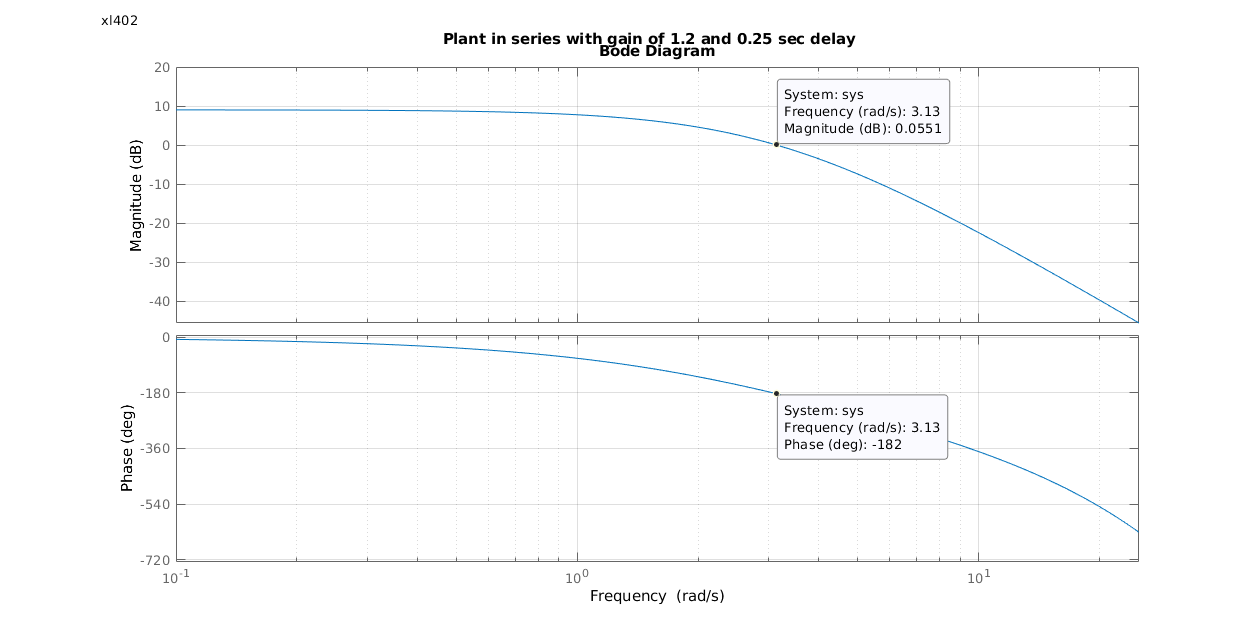
\includegraphics[width=0.9\linewidth]{2_PIO_Bode_Plot.png}
	\caption{PIO system open loop Bode plot}
	\label{fig:pio_bode}
\end{figure}

\begin{figure}[htp]
\centering
\begin{subfigure}{.5\textwidth}
  \centering
  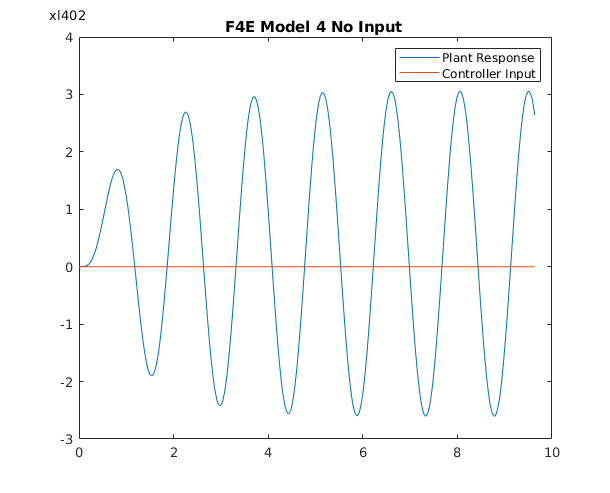
\includegraphics[width=0.9\linewidth]{2_3_F4E_Model_4_No_Input.png}
	\caption{Typical pilot plant PIO responses}
	\label{fig:f4e_no_input}
\end{subfigure}%
\begin{subfigure}{.5\textwidth}
  \centering
  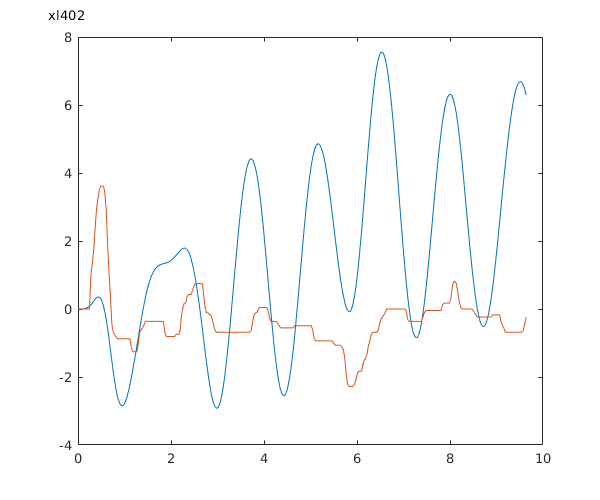
\includegraphics[width=0.9\linewidth]{2_3_F4E_Model_4_Manual_Control.png}
  \caption{Typical manual pilot-plant responses}
  \label{fig:f4e_response}
\end{subfigure}
\caption{F4E Model 4 fighter aircraft Responses}
\end{figure}

\section{Sinusoidal Disturbances Over F4E Fighter Aircraft}

Some more realistic models of the F4E fighter aircraft is analysed, there are four models representing the open loop dynamics, linearised about 4 different operating points (different altitudes and Mach numbers). As three models out of four are naturally unstable, only the fourth operating point is examined here (\textit{altitude=35000ft. Mach 1.5}).\\
Given a sinusoidal disturbance of $0.66Hz$ of magnitude 1, figure \ref{fig:f4e_no_input} shows the aircraft's responses without any pilot input. figure \ref{fig:f4e_response} shows its behaviour when the pilot attempts to stabalize it manually, with a gain of 1, and a time delay $D$ calculate previously. Clearly, the pilot is unable to reduce the oscillation of the aircraft. The open loop Bode plot is shown in figure \ref{fig:f4e_bode}. From this we can calculate the maximum proportional gfain for which the closed system is stable, reading from the $-180$ line, we find that for a gain of 1, the aircraft is in fact unstable (above $0dB$), the gain margin is actually $0.11$. This is confirmed from figure \ref{fig:f4e_response} as the pilot is more careful at using the joystick. Also the gain and phase and gain at $0.66Hz=4.14\textrm{rad/s}$ is $9.03dB$ and $-164\; \textrm{degrees}$ respectively. For a plant transfer function of $G$ and a controller transfer function of $K$, the open loop transfer function from $d$ to $y$ is simply $G$ as the reference signal $r$ is zero. For the closed loop transfer function $L$:
\begin{equation}
	L = \dfrac{G}{1+KG}
\end{equation}
\begin{figure}[htp]
	\centering
	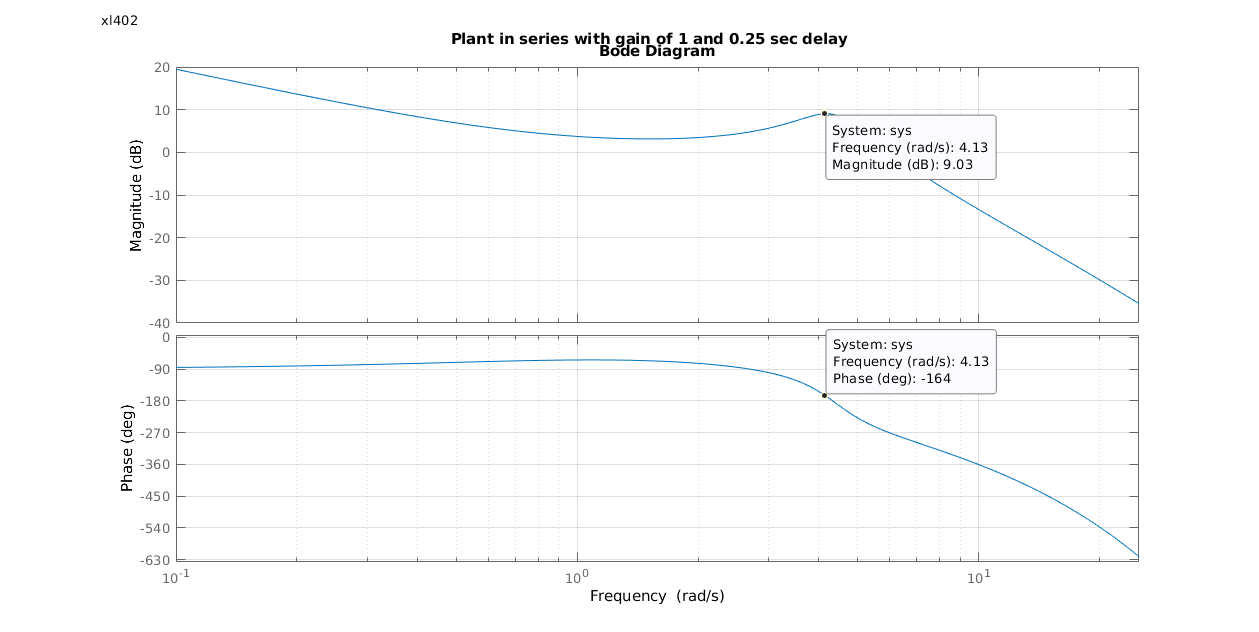
\includegraphics[width=\linewidth]{2_4_F4E_Model_4_Bode.png}
	\caption{F4E Model 4 open loop Bode plot}
	\label{fig:f4e_bode}
\end{figure}

\section{Unstable Aircraft Behaviour Analysis}
The behaviour of a unstable aircraft is investigated, taking the simplified model:
\begin{equation}
	G(s)=\dfrac{2}{sT-1}
\end{equation}
Which has an unstable at $1/T$, manual control with some trial and errors can achieve the stabalisation of this model with $T=0.5$ for full 5 seconds. The response of the pilot-plant response is shown in \ref{fig:unstable_response}. The nyquist diagram is shown in figure \ref{fig:unstable_nyquist}, we can see that there is a circle with anti-clockwise encirclement of the $-1$ point, therefore the plant itself is unstable, the nyquist plot reaches the x-axis at $-2$ point, therefore a proportional gain greater than $1/2$ will be able to stabalise this aircraft. The orange line indicated on the same graph is the time delayed (0.1 seconds) nyquist plot of the same plant, we can see that the gain required to stabalise it does not change.

\begin{figure}[htp]
\centering
\begin{subfigure}{.5\textwidth}
  \centering
  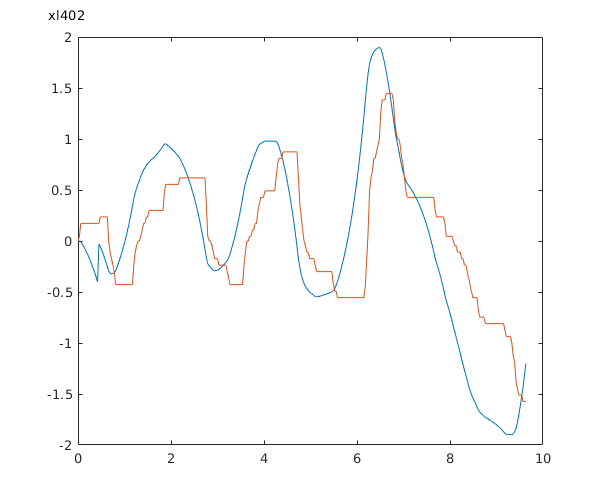
\includegraphics[width=\linewidth]{2_5_unstable_aircraft_response.png}
	\caption{Typical manual stabalisation response}
	\label{fig:unstable_response}
\end{subfigure}%
\begin{subfigure}{.5\textwidth}
  \centering
  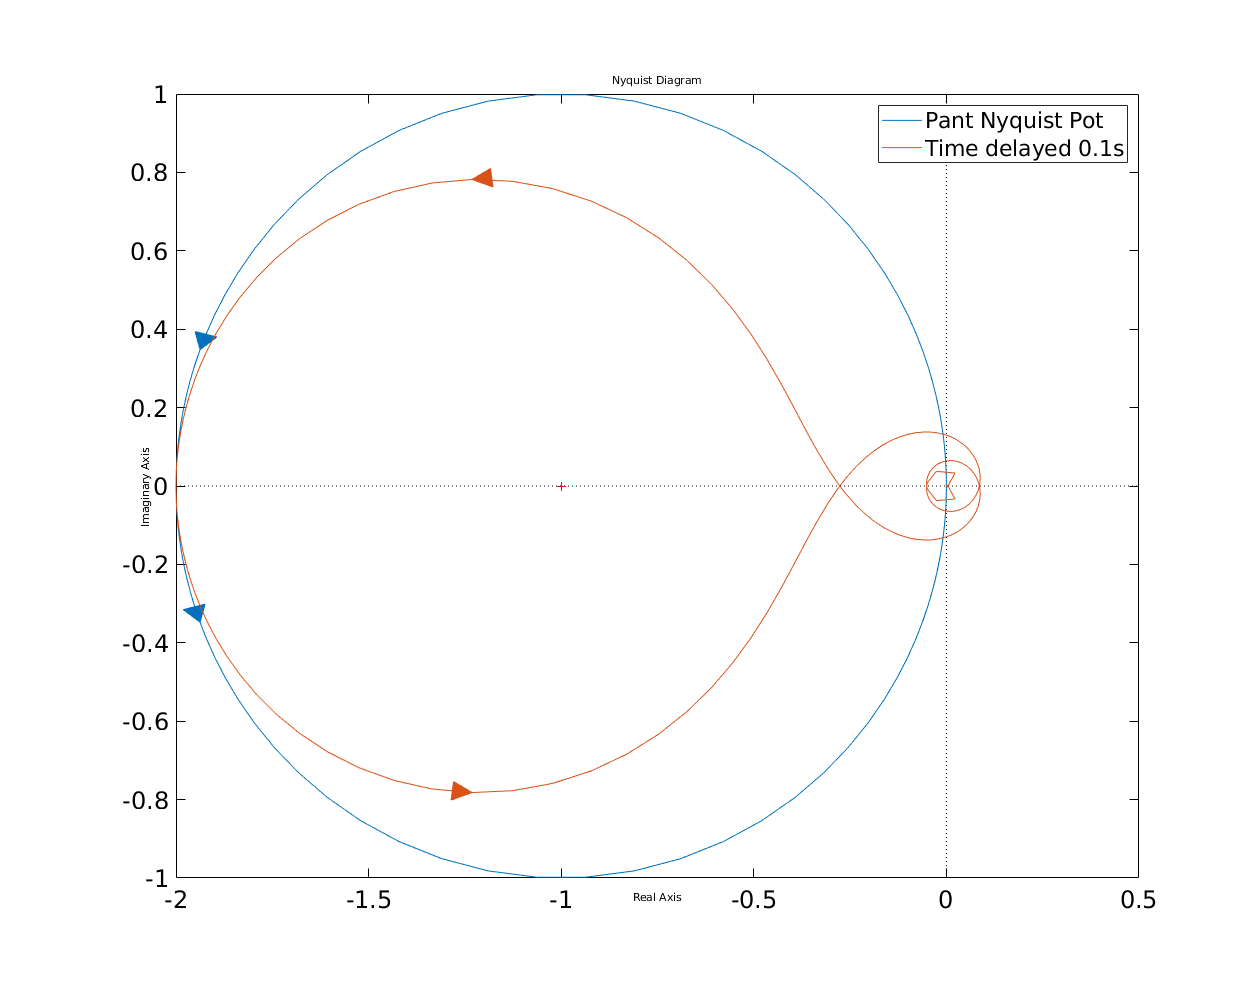
\includegraphics[width=1.08\linewidth]{unstable_nyquist.png}
  \caption{Open loop nyquist plot}
  \label{fig:unstable_nyquist}
\end{subfigure}
\caption{Unstable aircraft behaviour}
\end{figure}

\section{Autopilot}
Consider the following model for a transport aircraft on approach to landing:
\begin{equation}
	G_3(s=\dfrac{6.3s^2+4.3s+0.28}{s^5+11.2s^4+19.6s^3+16.2s^2+0.91s+0.27}
\end{equation}
The response of this aircraft model to an impulse disturbance of weight 2 is shown in figure \ref{fig:transport_noinput}. We devise a simple proportional negative feedback controller with gain of 5. This controller is tested with a disturbance impulse of weight 2 and a runtime of 15 seconds. It is observed that the oscillatary response disappears. The gain is slowly interesed until $K_c=17$ where the closed loop system begins to oscillate at a period of $1.81$ seconds.Therefore the gain margin of the loop when a proportional controller with a gain of 5 is used is $17/5=3.4=10.62dB$.
\begin{figure}[htp]
\centering
\begin{subfigure}{.5\textwidth}
  \centering
  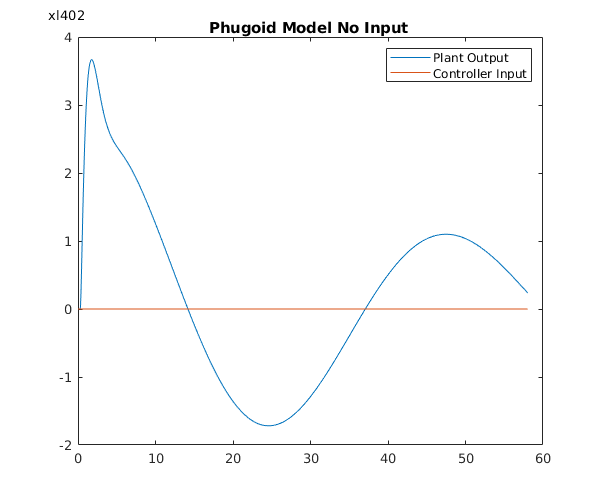
\includegraphics[width=0.9\linewidth]{3_1_phygoid_Model_no_input.png}
	\caption{No input impulse response}
	\label{fig:transport_noinput}
\end{subfigure}%
\begin{subfigure}{.5\textwidth}
  \centering
  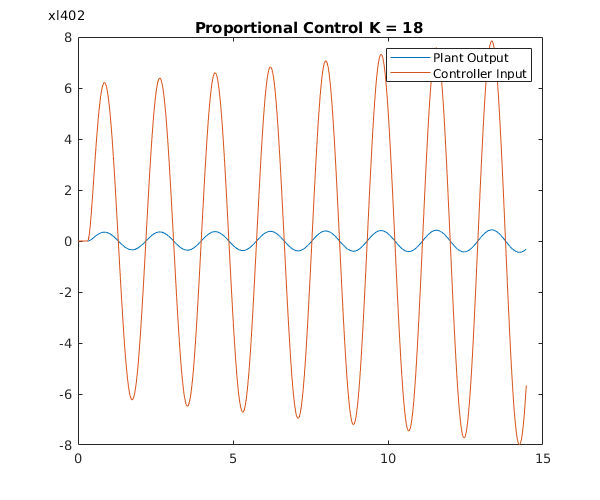
\includegraphics[width=0.9\linewidth]{3_2_autopilot.png}
  \caption{Oscillatary response at high gain}
  \label{fig:transport_osci}
\end{subfigure}
\caption{Proportional control of transport aircraft}
\end{figure}

\section{PID Controller}
The autopilot is to be implemented with a proportional-integral-derivative (PID) controller of the form:
\begin{equation}
	u(t)=K_p \left( e(t) + \dfrac{1}{T_i}\int_0^t e(\tau) d\tau + T_d \dfrac{de}{dt}\right)
\end{equation}
The transfer function of this controller is therefore:
\begin{equation}
	K = \dfrac{K_p(1+sT_i+s^2T_iT_d)}{sT_i}
\end{equation}
According to the \textit{Zeigler-Nichols} rules in process control, the parameters should be set as:
\begin{equation}
	K_p=0.6K_c, \quad T_i=0.5T_c, \quad T_d=0.125T_c
\end{equation}
In our case following $T_c$ (time period of proportional feedback induced oscillation) and $K_c$ (maximum feedback gain before oscillation) fom the section above, $K_p=0.6\times 17=10.2$, $T_i=0.5\times1.81=0.905$ and $T_d=0.125\times1.81=0.226$. Figure \ref{fig:pid_std} shows the response after implementing such feedback system, figure \ref{cw_25} shows the response after increasing the gain by 40\%, note the slight increase in damping (reduced oscillation).

\begin{figure}[htp]
\centering
\begin{subfigure}{.5\textwidth}
  \centering
  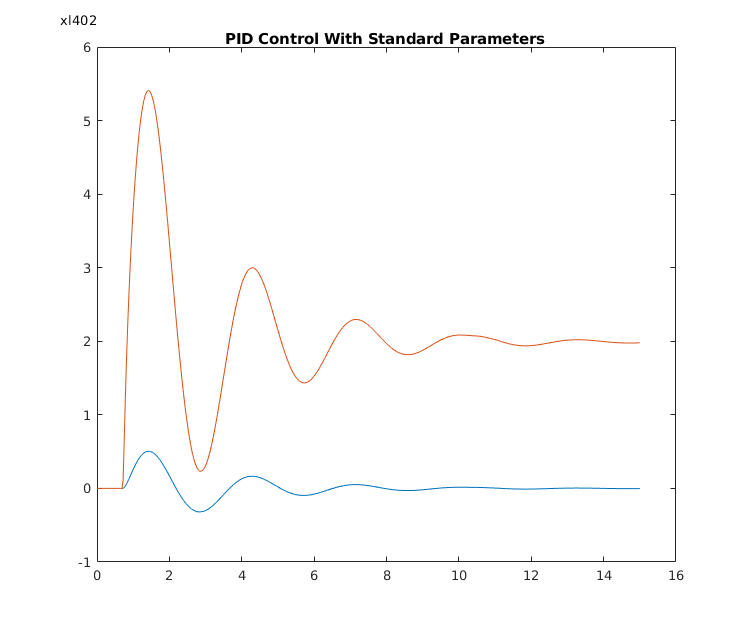
\includegraphics[width=0.9\linewidth]{PID_control_std.png}
	\caption{Standard Ziegler-Nichols parameters}
	\label{fig:pid_std}
\end{subfigure}%
\begin{subfigure}{.5\textwidth}
  \centering
  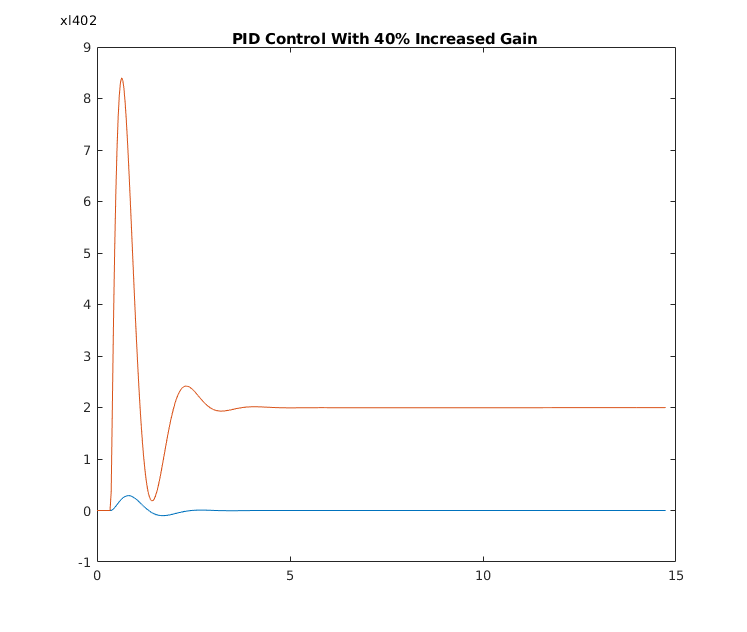
\includegraphics[width=0.9\linewidth]{PID_control_40percent.png}
  \caption{Increased gain (40\%)}
  \label{fig:cw_25}
\end{subfigure}
\caption{PID Controlled aircraft response}
\end{figure}


\section{Integrator Wind-Up}
When the disturbance is set to a high impulse, a phenomena called the integrator wind-up is observed, this can cause unwanted overshoot/undershoot after a period of input saturation due to the integrator being 'wound up' and having to unload again. One simple corrective method is to set a limit on the integrator. Figure \ref{fig:wind} shows this issue, note how it takes the controller several large swings to stabalise the aircraft. Figure \ref{fig:wind_fixed} shows the outcome of setting a threshold of the integrator. Following the code given, the smallest number which guarantees a zero steady-state error in response to a step disturbance of weight 2 is $0.1$.

\begin{figure}[htp]
\centering
\begin{subfigure}{.5\textwidth}
  \centering
  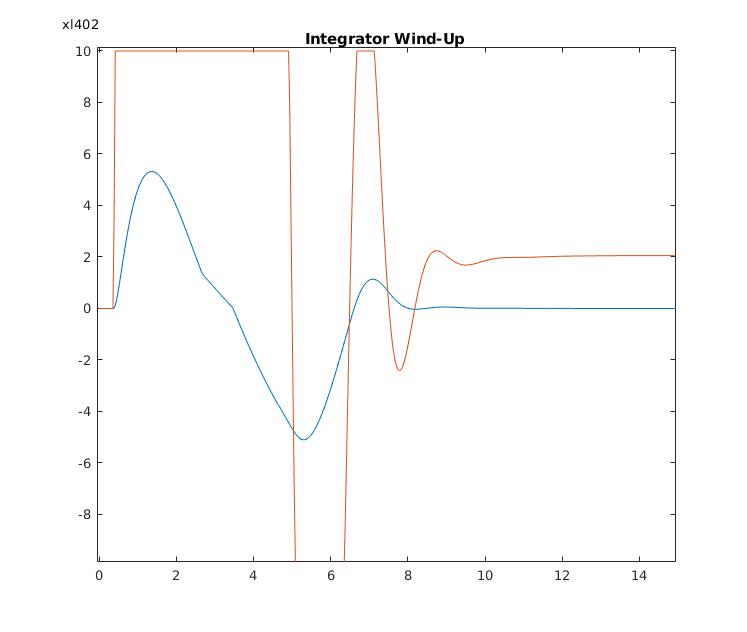
\includegraphics[width=0.9\linewidth]{wind_up.png}
	\caption{Integrator wind-up issue}
	\label{fig:wind}
\end{subfigure}%
\begin{subfigure}{.5\textwidth}
  \centering
  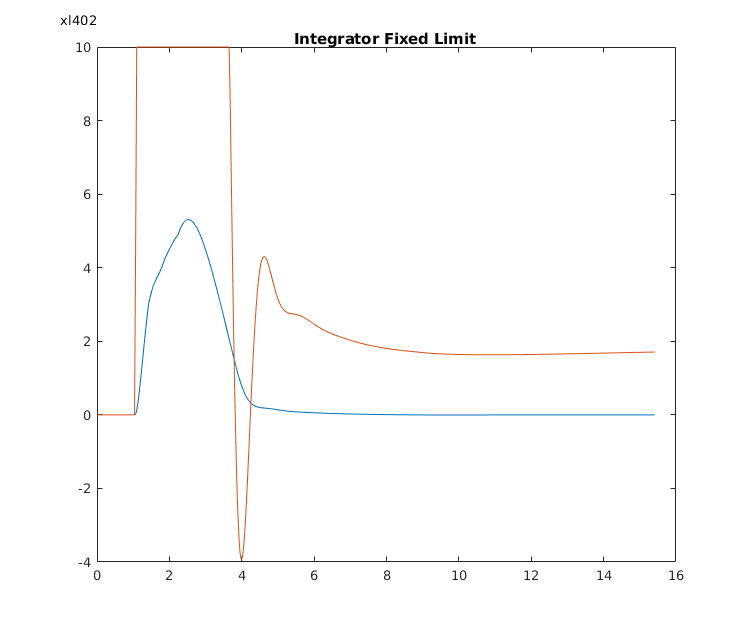
\includegraphics[width=0.9\linewidth]{wind_up_fixed.png}
  \caption{Integrator limit set}
  \label{fig:wind_fixed}
\end{subfigure}
\caption{Aircraft response over large disturbance}
\end{figure}

\section{Appendix: MATLAB Code}
Code below is from the \textit{flysim1.m} file:
\begin{lstlisting}
num=[6.3 4.3 0.28];
den=[1 11.2 19.6 16.2 0.91 0.27];

runtime=15;
wght=[0,1,5,0.66];

samper=30;

srate=(samper+1.3)/1000;

grphc1

integ=0;deriv=0;yprev=0;
Kp=10.2*1.7; Ti=0.98; Td=0.4;
for i=1:count
	set(hh,'Xdata',hx,'Ydata',hy+y*hz);
    integ = integ+0.5*(y+yprev)*srate;
    integ=sign(integ)*min(abs(integ),0.10);
    deriv=(y-yprev)/srate;
    pp=-Kp*(y+integ/Ti+deriv*Td);
    yprev=y;
	pp=sign(pp)*min(max(0,abs(pp)-0.0),10);

	set(jh,'Xdata',jx,'Ydata',jy+pp*jz);
	drawnow;

	ylist(i)=y;
	ulist(i)=pp;

	x=adis*x + bdis*(pp+disturb(i));
	y=cdis*x + ddis*(pp+disturb(i));

	while (time2-time1<samper)
		time2=clock;time2=1000*(60*time2(5)+time2(6));
	end
	thetimes(i)=time2;
	time1=time2;

	if (y<-10 | y>10 )
		flg=1;crashind=i+1;
		thetimes(i+1)=thetimes(i)+samper;
		ylist(i+1)=y;
		ulist(i+1)=sign(p(1,2))*min(abs(p(1,2)),10);
		break;
	end

end

grphc2
\end{lstlisting}

\end{document}
